% Course cover: generated cell illustration and two real scientific photographs.
% Image provenance and reuse terms: Lecture_Summaries/cover_image_sources.md.
\begin{titlepage}
\thispagestyle{empty}
\begin{tikzpicture}[remember picture,overlay]
\fill[primary!2] (current page.south west) rectangle (current page.north east);
\fill[primary] (current page.north west)
  rectangle ([yshift=-186mm]current page.north east);
\fill[exacol] ([yshift=-186mm]current page.north west)
  rectangle ([yshift=-188mm]current page.north east);
\node[anchor=north west,text=white!80,font=\small\sffamily,
  text width=155mm,align=left]
  at ([xshift=25mm,yshift=-21mm]current page.north west)
  {THE HEBREW UNIVERSITY OF JERUSALEM\\[3pt]Racah Institute of Physics};
\node[anchor=north west,text=white,font=\small\sffamily\bfseries]
  at ([xshift=25mm,yshift=-41mm]current page.north west)
  {COURSE 77972};
\node[anchor=north west,text=white,text width=160mm,align=left,
  font=\fontsize{29}{35}\selectfont\bfseries]
  at ([xshift=25mm,yshift=-54mm]current page.north west)
  {Physical Models of\\Biological Systems};
\node[anchor=north west,text=white!85,font=\large]
  at ([xshift=25mm,yshift=-91mm]current page.north west)
  {Lecture summaries \enspace\textbullet\enspace Exam revision};
% Native 1024 x 1536 illustration: 55 mm tall gives approximately 709 ppi.
\node[inner sep=0pt] at ([xshift=50mm,yshift=-140mm]current page.north west)
  {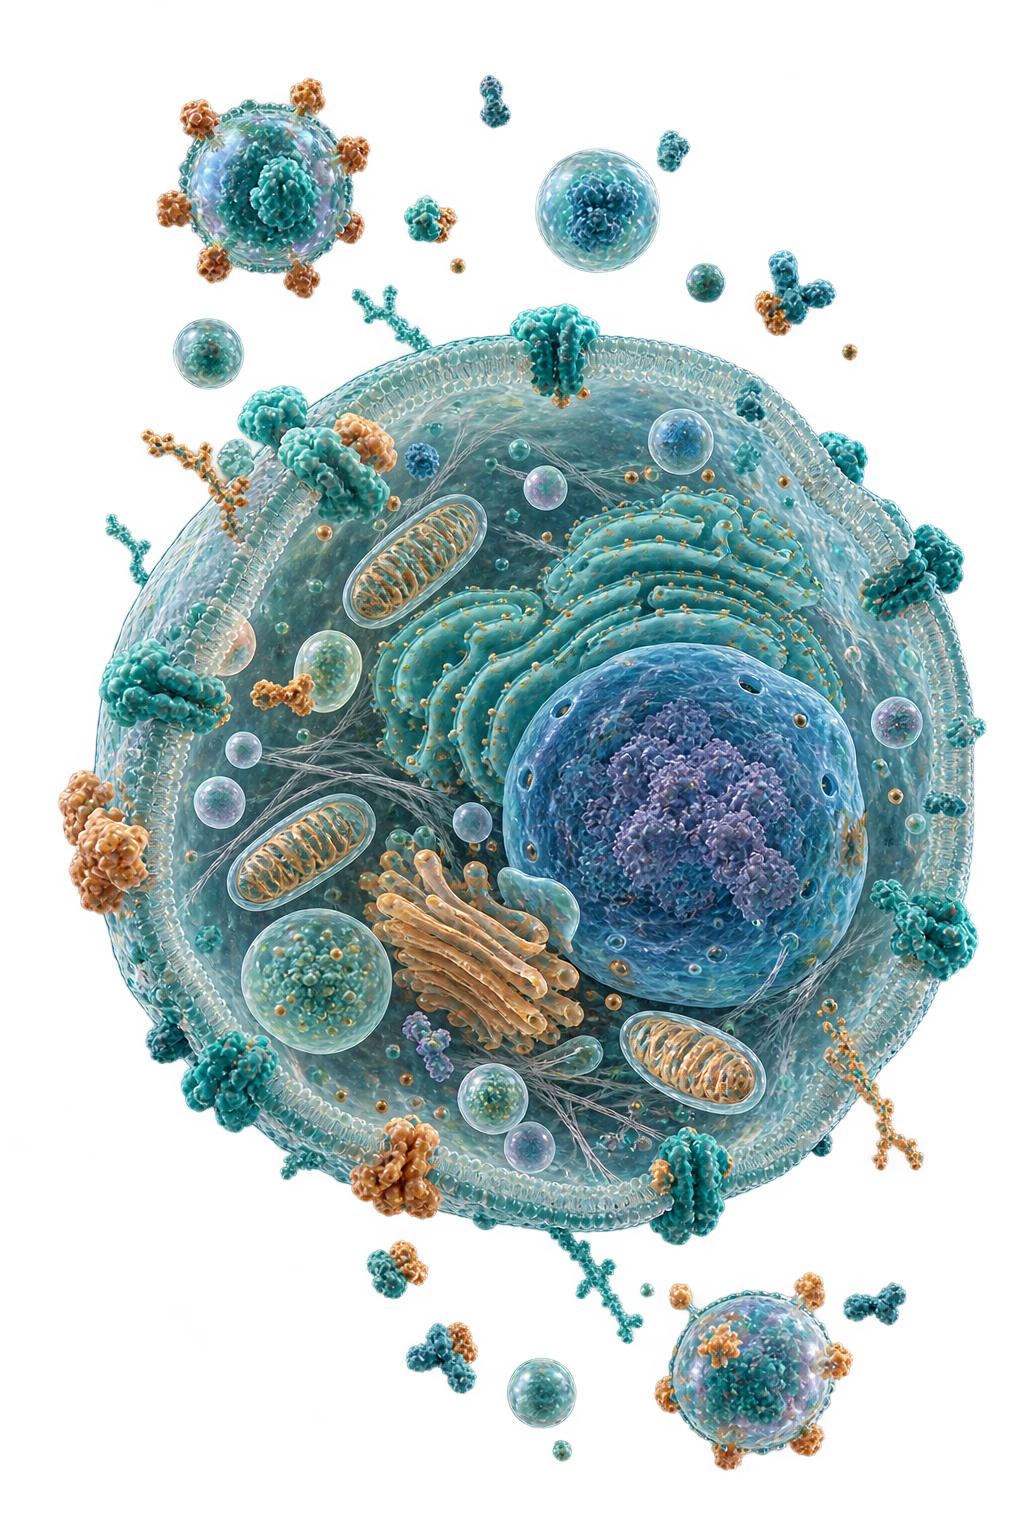
\includegraphics[height=55mm]{Lecture_Summaries/cover_biological_systems.png}};
% Original branching-colony photograph supplied by the user; no recoloring.
\node[inner sep=0pt] at ([xshift=105mm,yshift=-140mm]current page.north west)
  {\includegraphics[width=50mm]{Lecture_Summaries/cover_branching_colony.jpg}};
% Layout-only square crop of the original NOAA photograph; no recoloring.
\begin{scope}
\clip ([xshift=135mm,yshift=-115mm]current page.north west)
  rectangle ([xshift=185mm,yshift=-165mm]current page.north west);
\node[inner sep=0pt] at ([xshift=160mm,yshift=-140mm]current page.north west)
  {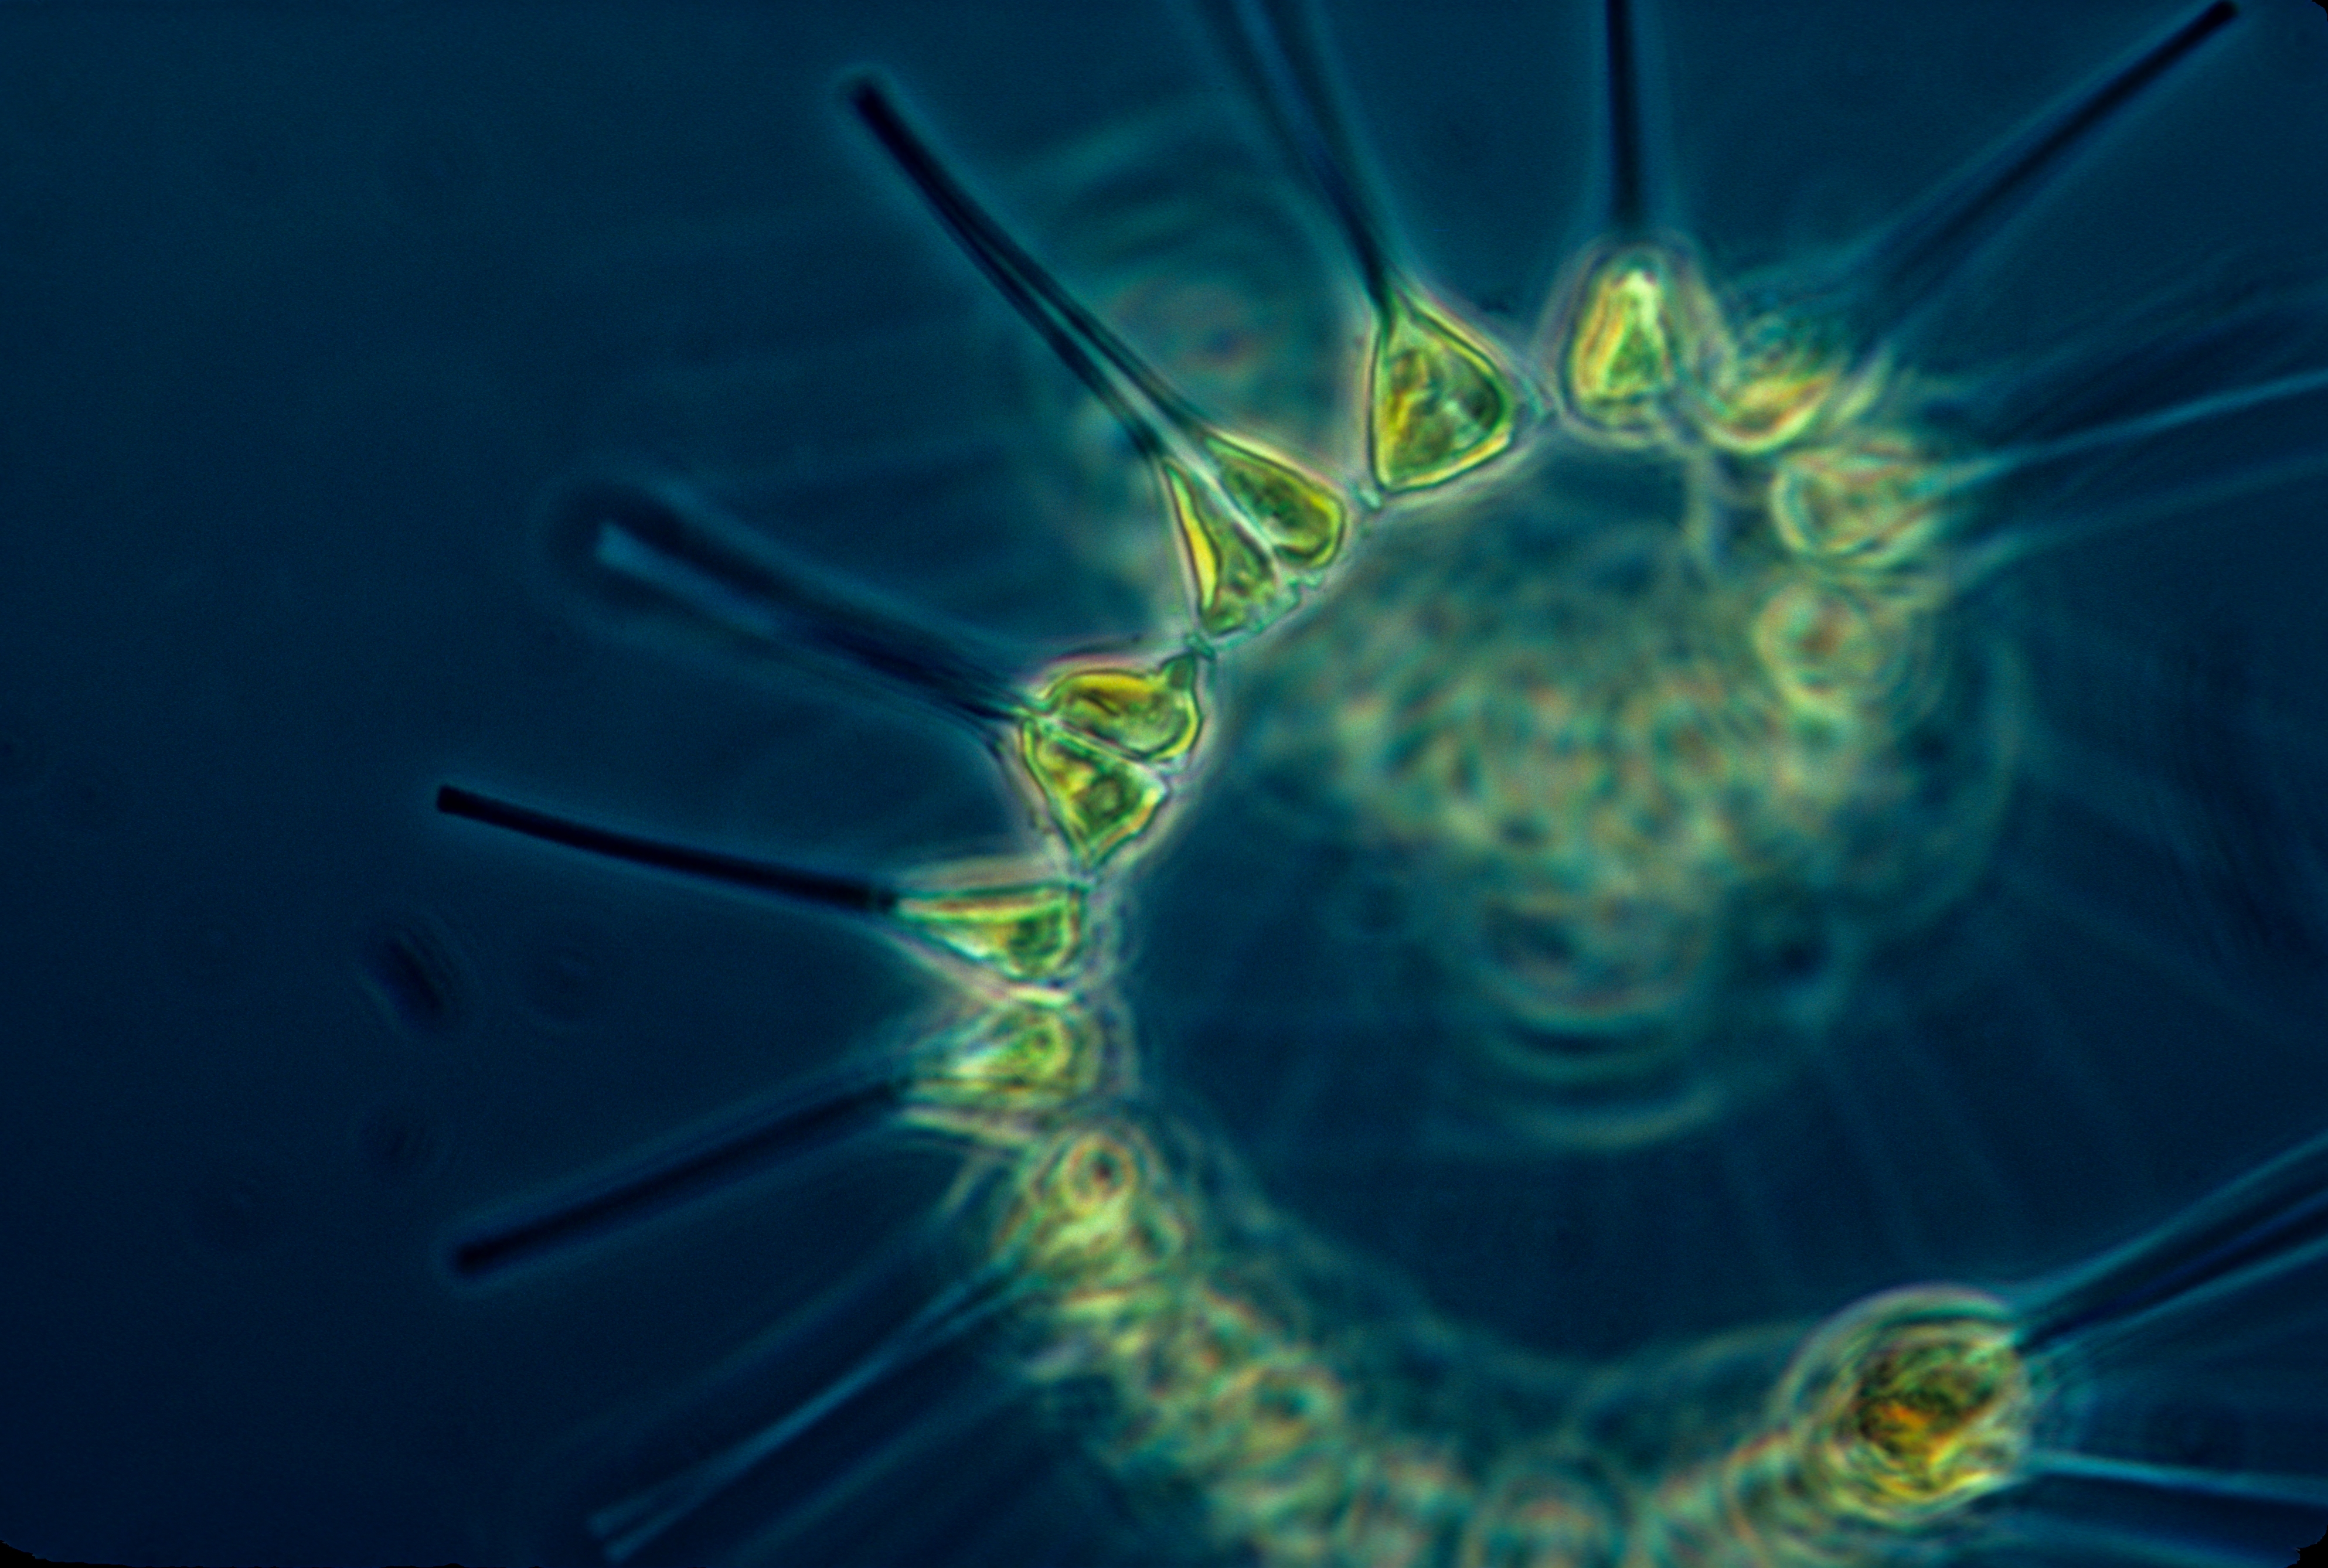
\includegraphics[height=50mm]{Lecture_Summaries/cover_plankton.jpg}};
\end{scope}
\foreach \x/\caption in {50/Cellular mechanisms,105/Microbial populations,160/Phytoplankton}
  \node[text=white!85,font=\small\sffamily]
    at ([xshift=\x mm,yshift=-175mm]current page.north west) {\caption};
\node[anchor=north west,text=primary,font=\large\bfseries]
  at ([xshift=25mm,yshift=-200mm]current page.north west)
  {2026--2027 \enspace|\enspace Semester A};
\node[anchor=north west,text=primary!85!black,align=left,
  font=\normalsize,inner sep=0pt]
  at ([xshift=25mm,yshift=-218mm]current page.north west)
  {\begin{tabular}{@{}ll@{}}
    \textbf{Lecturer} & Dr. Amir Erez\\[8pt]
    \textbf{Notes prepared by} & \summaryauthor
  \end{tabular}};
\node[anchor=north west,text=primary!80!black,font=\scriptsize,
  text width=155mm,align=left,inner sep=0pt]
  at ([xshift=25mm,yshift=-257mm]current page.north west)
  {Cover: AI-generated conceptual cell illustration; branching colony:
   \href{https://commons.wikimedia.org/wiki/File:Microscope_view_of_a_branched_Bacillus_bacterial_colony_08.jpg}{Korinna (2020)},
   \href{https://creativecommons.org/licenses/by/4.0/}{CC BY 4.0};
   phytoplankton: NOAA MESA Project, NOAA Photo Library, public domain, cropped.};
\draw[primary!25,line width=0.5pt]
  ([xshift=25mm,yshift=19mm]current page.south west)--
  ([xshift=-25mm,yshift=19mm]current page.south east);
\node[anchor=south west,text=primary!75,font=\small,text width=155mm]
  at ([xshift=25mm,yshift=10mm]current page.south west)
  {Personal revision notes based on lectures and course materials.};
\end{tikzpicture}
\null
\end{titlepage}
